\chapter{Simulationen von kristallinem und amorphem Silizium}
\label{appendix_silicon}

Die Bindungslängen für verschiedene Parametrisierungen wurden direkt aus der ersten Spitze in der radialen Verteilungsfunktion für einen Silizium-Kristall nach einer thermischen Relaxierung ermittelt und in Abbildung~\ref{fig:sisibondlengths} zusammen gefasst.
Für die \pot{newsome}-Parametrisierung ergibt sich durch Aufspaltung der Hauptbindungslänge eine zusätzliche RDF-Spitze vor der eigentlichen Bindungslänge (Abbildung~\ref{fig:newsomerdf}), welche dadurch unterschätzt wird.
Darin zeigt sich eine Fehl\-para\-metri\-sierung des \pot{newsome}-Parametersatzes, welcher auf die Beschreibung von \ce{SiC}-Strukturen ausgelegt ist.
Für die anderen Parametersätze zeigen sich ansonsten gute Übereinstimmungen mit der Bindungslänge von \SI{2.3515}{\angstrom}\cite{haynes_crc_2011}.

\begin{figure}[p]
  \centering
  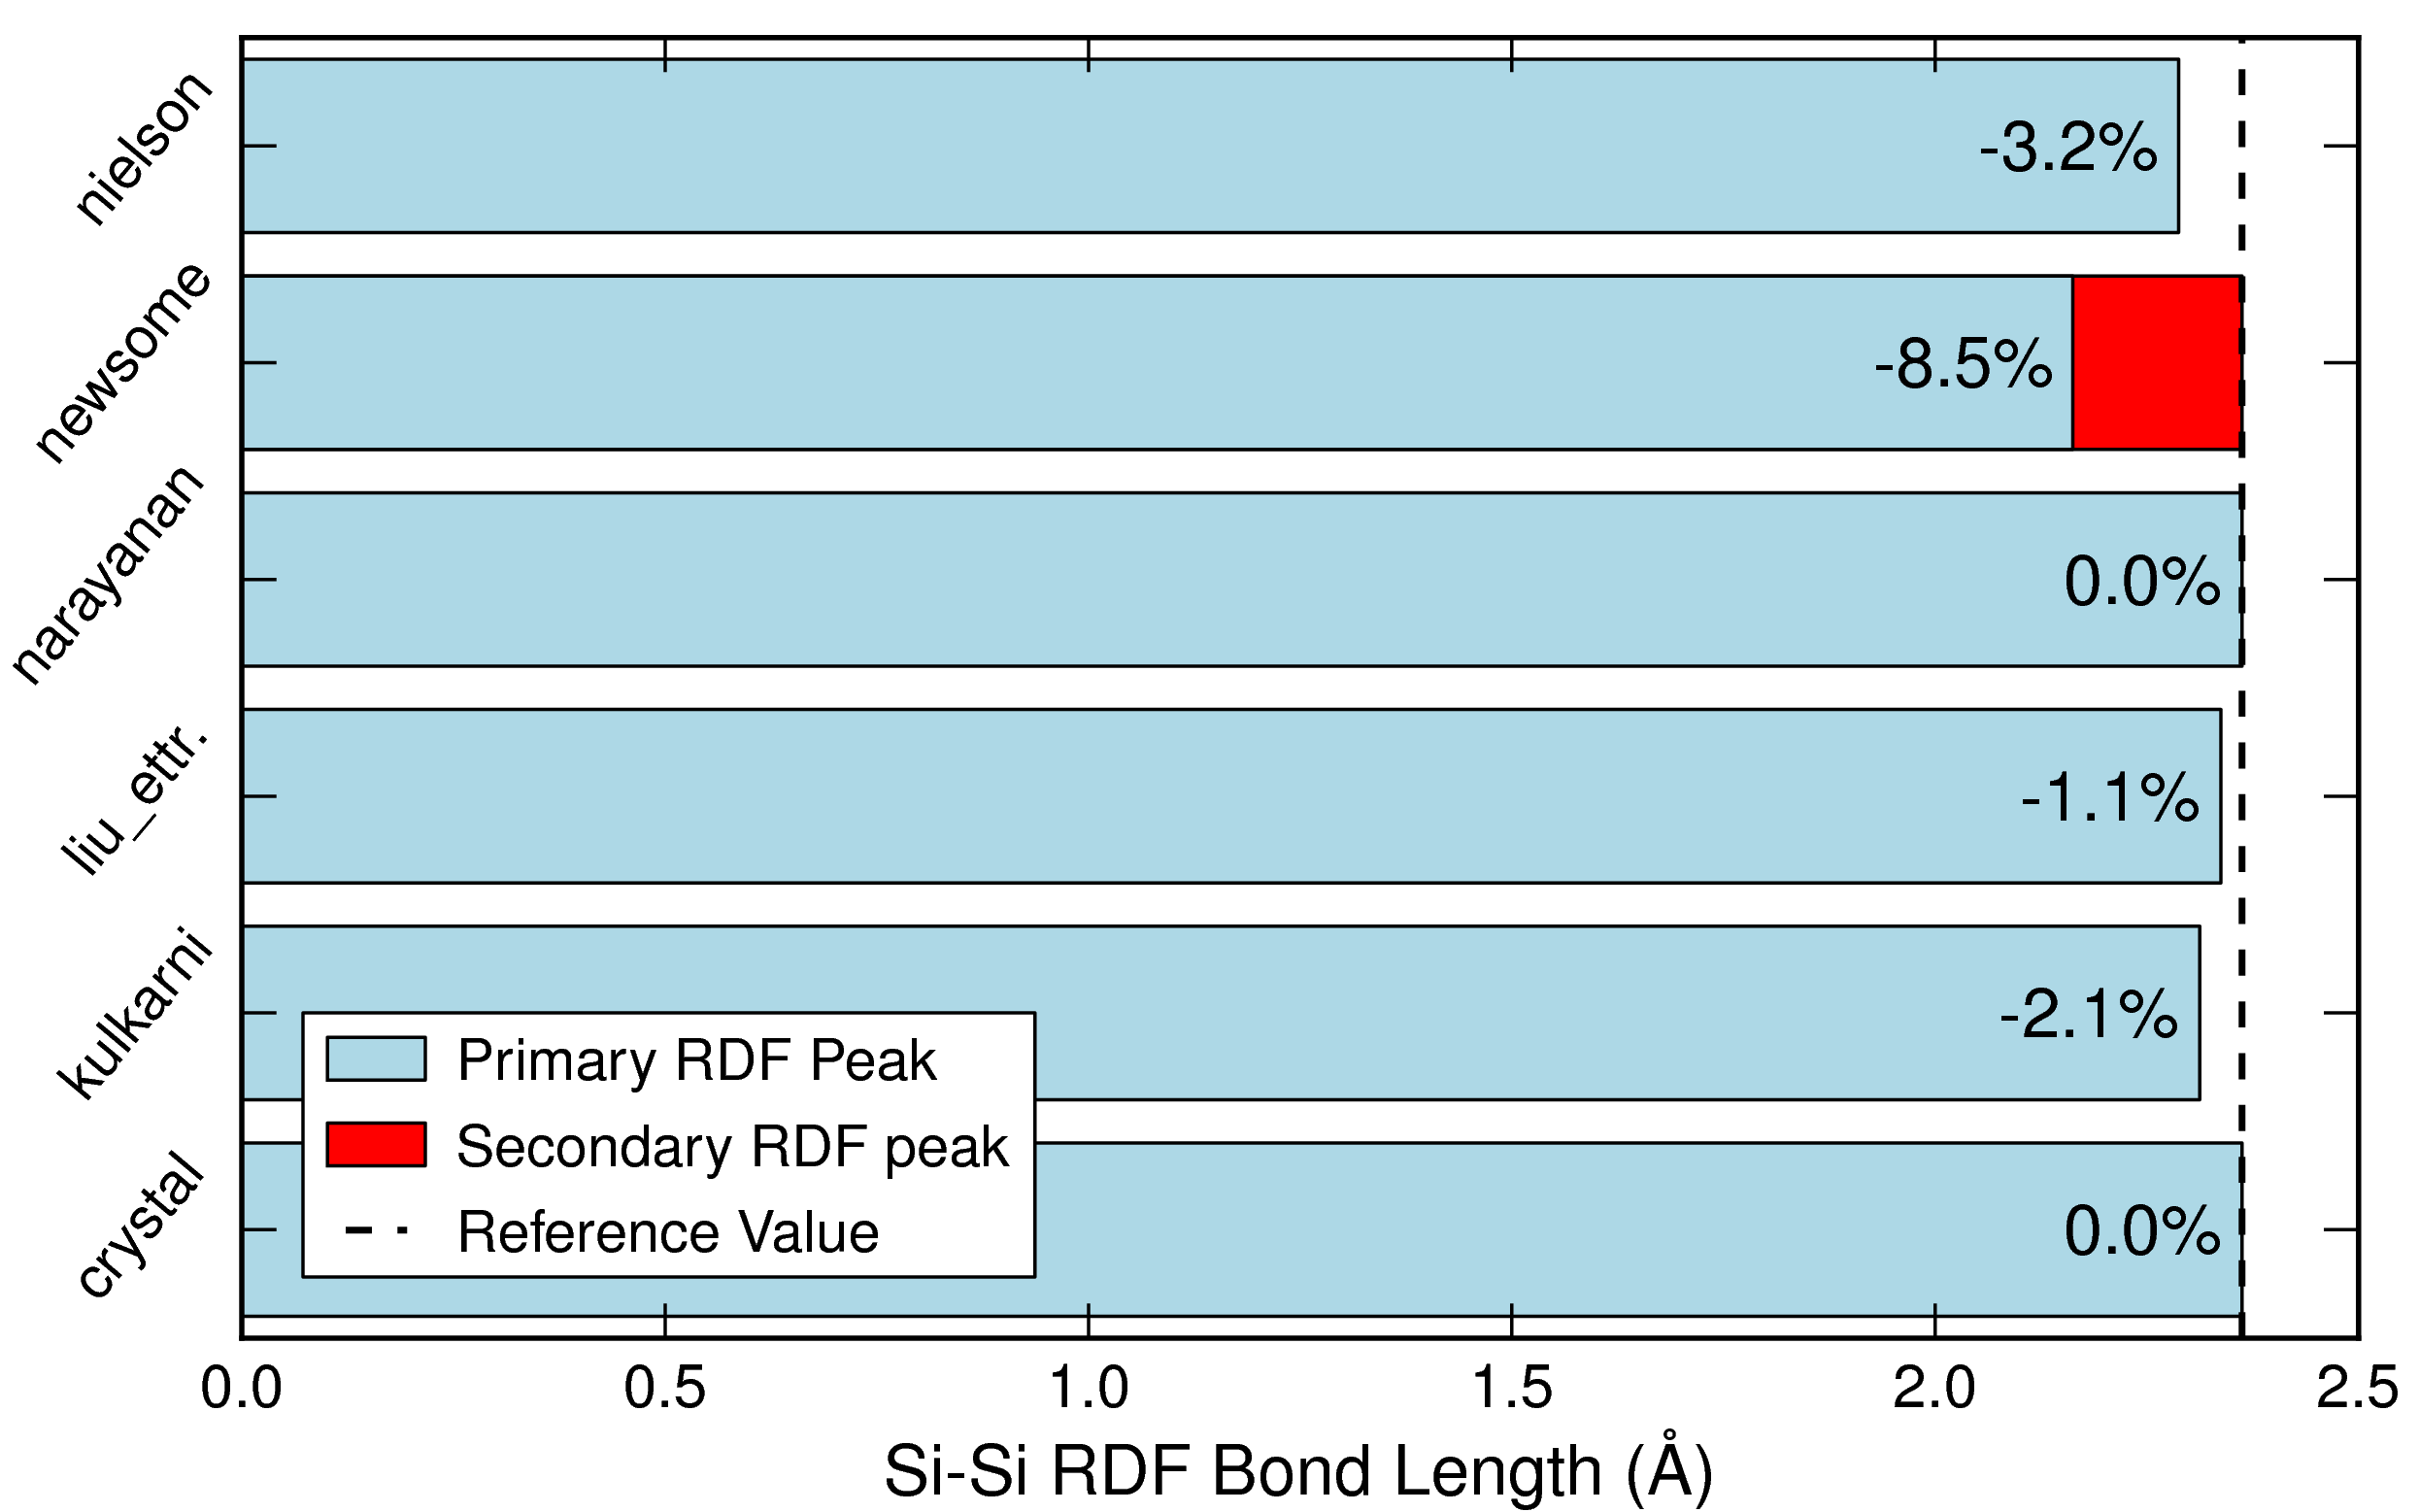
\includegraphics[width=10cm]{SiSi_npt_bondlengths}
  \caption{Bindungslängen von c-\ce{Si} für ReaxFF-Parametrisierungen}
  \label{fig:sisibondlengths}
\end{figure}

Bei Untersuchungen der RDF der Parametrisierungen hinsichtlich der Qualität der Kristalle zeigen mit Ausnahme der \pot{newsome}-Parametrisierung (Abbildung~\ref{fig:newsomerdf}) alle Parametersätze perfekte RDF-Spitzen entsprechend der kristallinen Struktur, nachdem diese sich durch thermische Bewegungen der Moleküle bei der Relaxierung verbreitert hatten.
Nachfolgend soll hauptsächlich die für die PVD-Simulationen genutzte \pot{kulkarni}-Parametrisierung untersucht werden, deren RDF in Abbildung~\ref{fig:kulkarnirdf}) abgebildet sind.
Im isotherm-isobaren Ensemble schrumpft mit ihr der Kristall zwar um \SI{2.1}{\percent}, behält seine Struktur aber ohne Einschränkung bei.

\vspace{2em}

\begin{figure}[H]
  \centering
  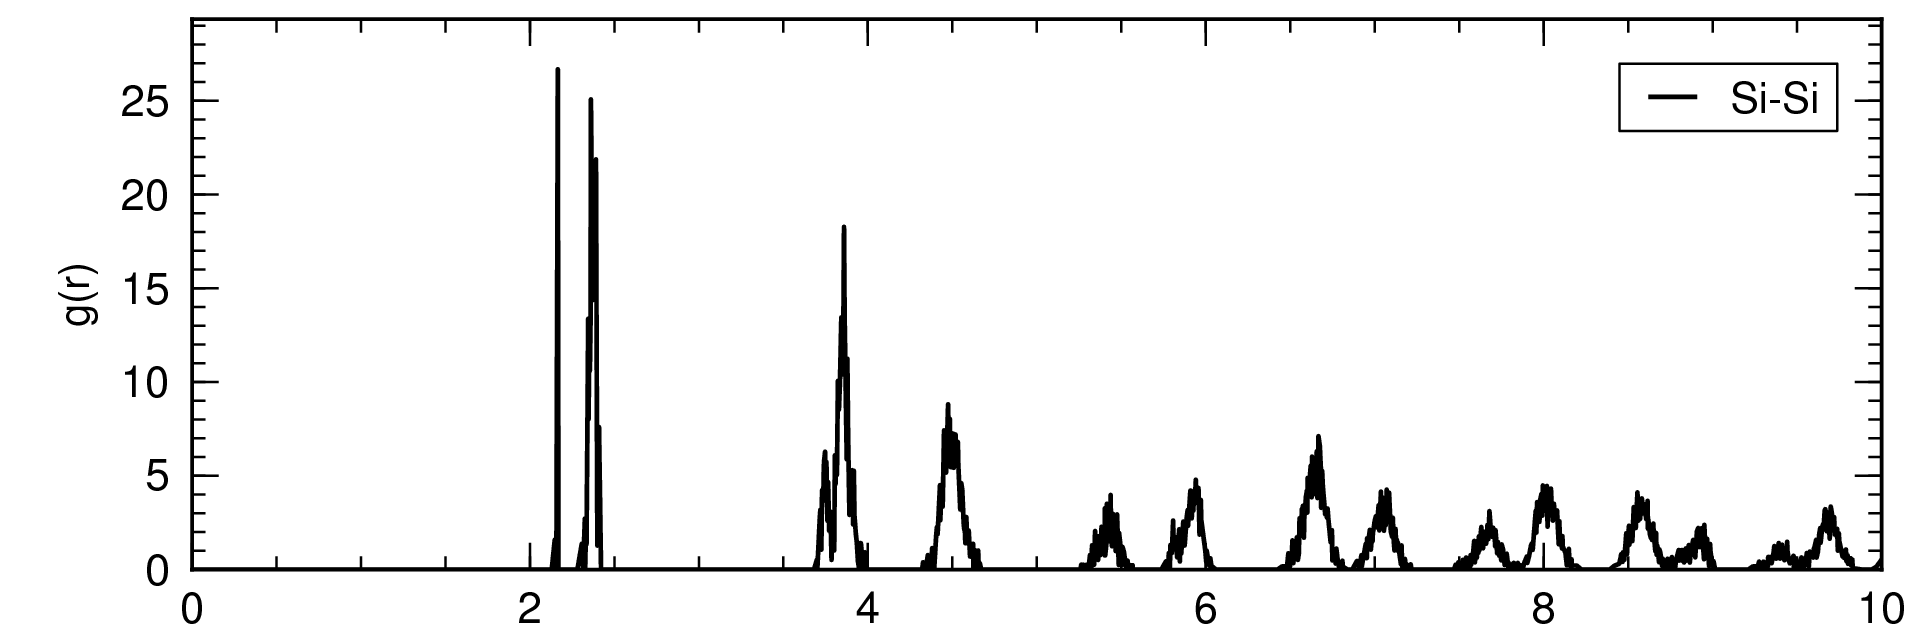
\includegraphics[width=\textwidth]{Si_newsome_rdf}
  \caption{Radiale Verteilungsfunktion mit \pot{newsome} nach Energieminimierung}
  \label{fig:newsomerdf}
\end{figure}


\begin{figure}[p]
  \centering
  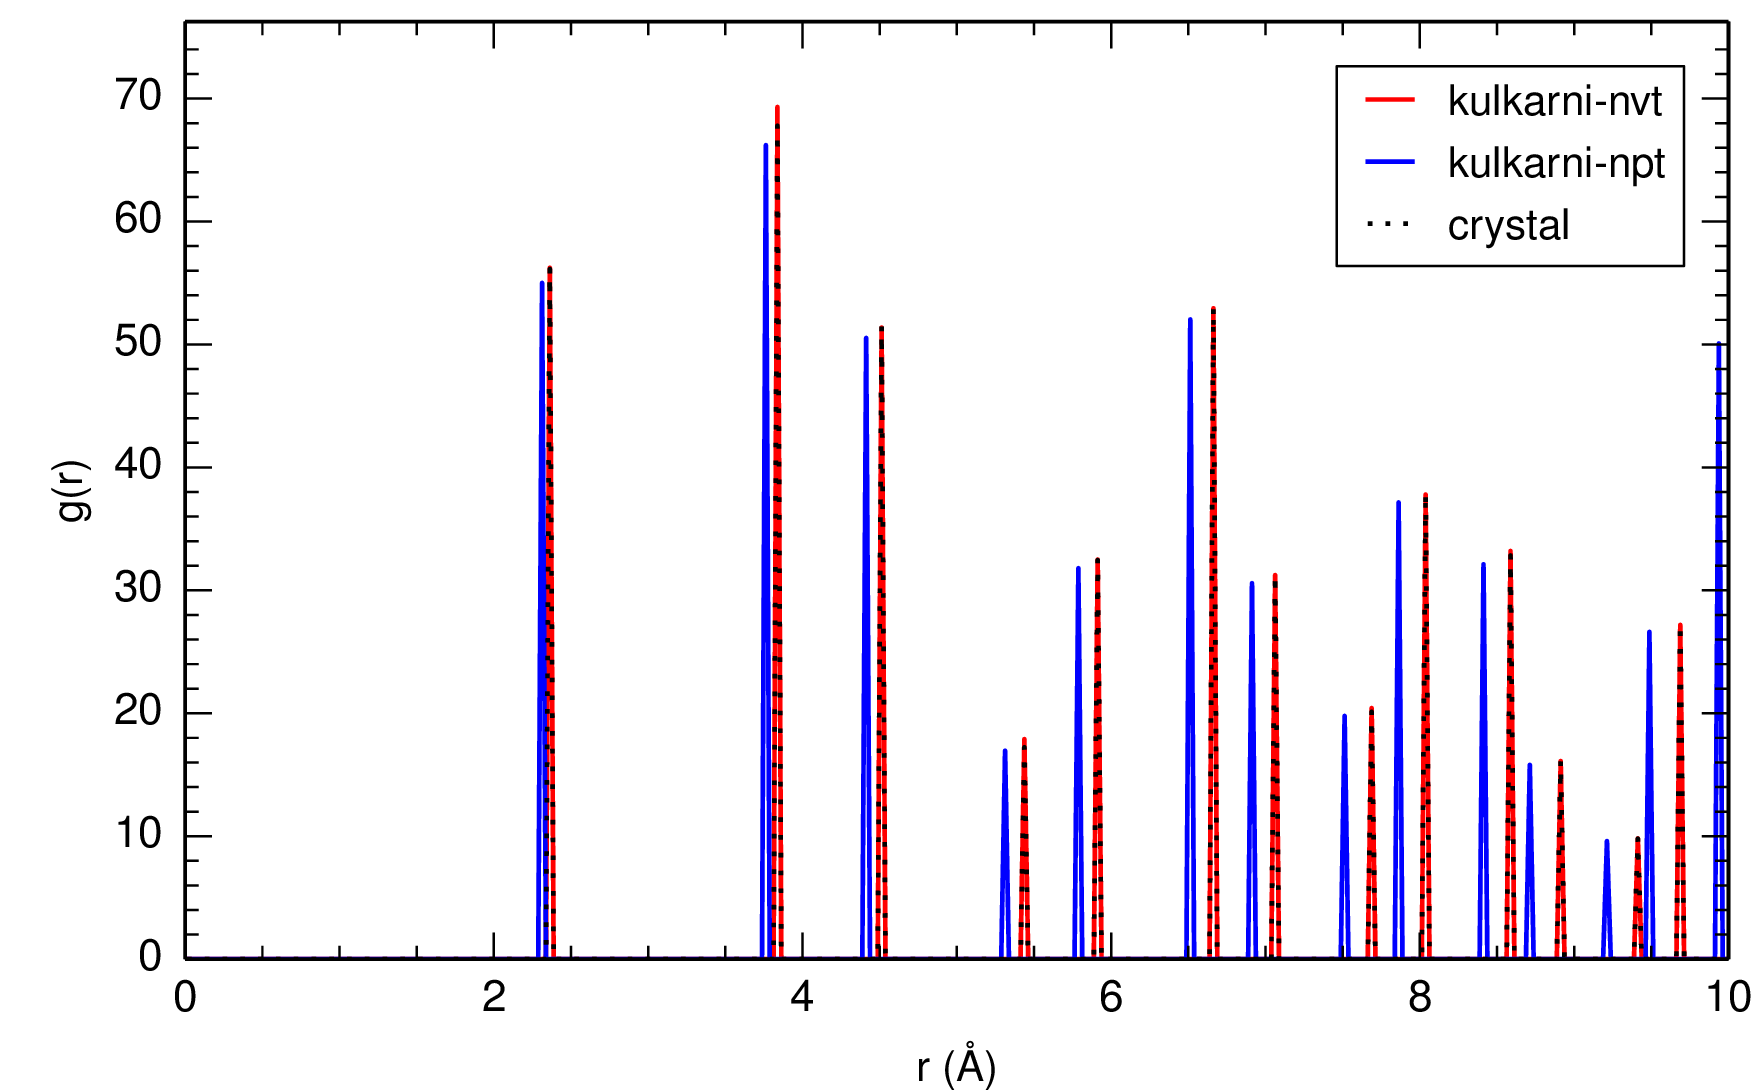
\includegraphics[width=\textwidth]{kulkarni_rdf_crystal}
  \caption[Radiale Verteilungsfunktionen von relaxiertem c-\ce{Si}]{
    Radiale Verteilungsfunktionen von relaxiertem c-\ce{Si} mit \pot{kulkarni}
  }
  \label{fig:kulkarnirdf}
\end{figure}

\clearpage

Die Untersuchung amorpher Siliziumstrukturen, die aus Simulationen der Relaxierung randomisierter Siliziumstrukturen im kanonischen Ensemble bei \SI{1500}{\kelvin} sowie aus der Simulation einer langsamen Abkühlung von geschmolzenem Silizium bei \SI{2000}{\kelvin} entstanden, zeigt sich keine Kristallisation bei den untersuchten Parametersätzen (\pot{kulkarni}: Abbildung~\ref{fig:amorphousrdf}).
Bereits nach \SI{4}{\angstrom} ist keine langreichweitige Ordnung erkennbar, doch ist die Bindungslänge klar erkennbar (\SI{2.339}{\angstrom} bei \pot{kulkarni}).
In Tabelle~\ref{tab:amorphoussilicon} sind die ermittelten strukturellen Werte für alle untersuchten Parametrisierungen zusammen gefasst.

\begin{figure}[H]
  \centering
  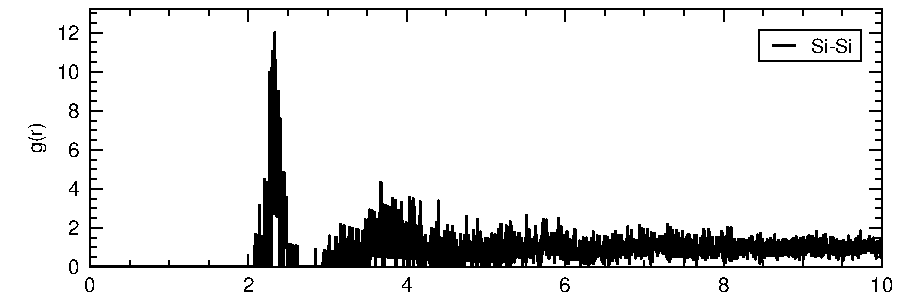
\includegraphics[width=13cm]{kulkarni_rdf_amorphous}
  \caption[Radiale Verteilungsfunktionen von relaxiertem a-\ce{Si}]{
    Radiale Verteilungsfunktionen von relaxiertem a-\ce{Si} mit \pot{kulkarni}
    }
  \label{fig:amorphousrdf}
\end{figure}

\begin{table}[H]
  \begin{threeparttable}

    \caption{Vergleich der Struktur amorphen Siliziums}
    \label{tab:amorphoussilicon}

    \oddrowcolors
    \begin{tabularx}{\textwidth}{|llXXlX|}
      \hline
      \textbf{Parametrisierung} & \multicolumn{2}{l}{\textbf{Bindungslänge}}   & \textbf{Koord.} & \textbf{Dichte}    & ~                        \\
      \hline
      (kristallin)              & \SI{2.352}{\angstrom} & ~                    & \num{4.00}      & \SI{2.3296}{\gpcc} & ~                        \\
      amorph                    & ~                     & ~                    & ~               & \SI{2.29}{\gpcc} \cite{remes_optical_1998} &  \\
      \pot{Al\_Al0\_AlN}        & \SI{2.379}{\angstrom} & \SI{+1.15}{\percent} & \num{4.59}      & \SI{2.373}{\gpcc}  & \SI{+3.62}{\percent}     \\
      \pot{kulkarni}            & \SI{2.339}{\angstrom} & \SI{-0.55}{\percent} & \num{4.05}      & \SI{2.361}{\gpcc}  & \SI{+3.10}{\percent}     \\
      \pot{liu\_ettr.}          & \SI{2.401}{\angstrom} & \SI{+2.08}{\percent} & \num{4.10}      & \SI{2.314}{\gpcc}  & \SI{+1.05}{\percent}     \\
      \pot{narayanan}           & \SI{2.383}{\angstrom} & \SI{+1.32}{\percent} & \num{4.05}      & \SI{2.365}{\gpcc}  & \SI{+3.28}{\percent}     \\
      \pot{newsome}             & \SI{2.153}{\angstrom} & \SI{-8.46}{\percent} & \num{1.17}      & \SI{2.398}{\gpcc}  & \SI{+4.72}{\percent}     \\
      \pot{nielson}             & \SI{2.411}{\angstrom} & \SI{+2.51}{\percent} & \num{4.82}      & \SI{2.358}{\gpcc}  & \SI{+2.97}{\percent}     \\
      \pot{zhang}               & \SI{2.357}{\angstrom} & \SI{+0.21}{\percent} & \num{4.39}      & \SI{2.329}{\gpcc}  & \SI{+1.70}{\percent}     \\
      \hline
    \end{tabularx}

  \end{threeparttable}
\end{table}

%% \section{Struktur der amorphen Schicht nach einer Parsivald-Simulation}

%% Die Rauheit der aufgewachsenen Schicht hängt stark mit der Bildung und dem Wachstum der Poren zusammen, wodurch das lineare Wachstum der Poren für einen linearen Anstieg der RMS-Rauheit sorgt.
%% Mit der Schließung der Poren ist eine schlagartige Reduktion der Rauheit zu erwarten, welcher sich gegen Ende der Simulation bereits andeutet, aber nicht mehr statt findet.
%% Simulationen über längere Zeiträume und größere Schichten sind notwendig, diesen Effekt näher zu charakterisieren

%% \begin{figure}[ht]
%%   \centering
%%   \captionsetup[subfigure]{singlelinecheck=false}
%%   \def\subfigwidth{0.48\textwidth}
%%   \begin{subfigure}[t]{\subfigwidth}
%%     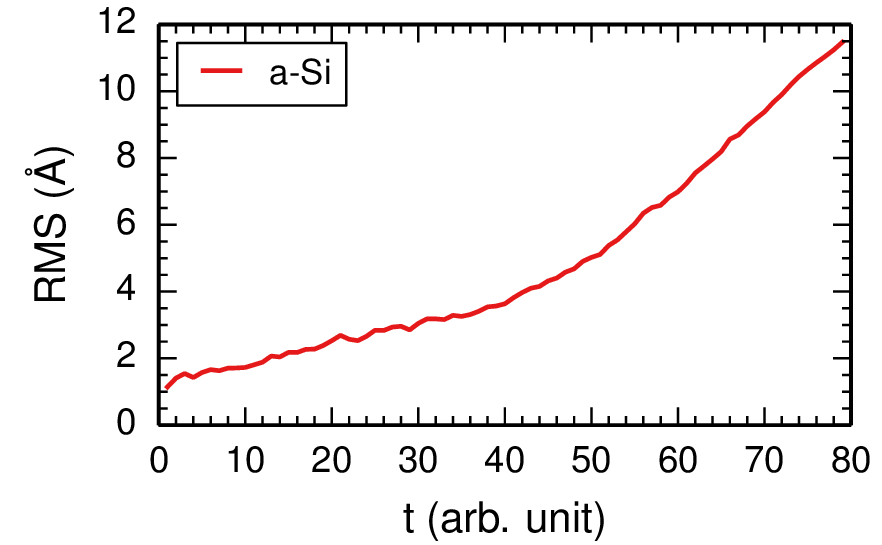
\includegraphics[width=\textwidth]{Si111_roughness}
%%     %% \subcaption{Dicke und Rauheit der Schicht}
%%     %% \label{fig:siliconresults-a}
%%   \end{subfigure}
%%   \caption{Zeitliche Entwicklung der Rauheit einer Silizium-PVD-Schicht}
%%   \label{fig:siliconroughness}
%% \end{figure}
